\documentclass{beamer}
\usepackage{tikz}
\usetikzlibrary{shapes}
\usetheme{Madrid}

\tikzstyle{startstop} = [ellipse,text centered,draw]
\tikzstyle{io} = [trapezium,trapezium left angle=70,trapezium right angle=110,text centered,draw]
\tikzstyle{normal} = [rectangle,text centered,text width=3cm,draw]
\tikzstyle{decision} = [diamond,text centered,aspect=3,draw]

\author[teacher]{class teacher}
\title[tikz and beamer]{practice on tikz and beamer}
\institute[BUET]{Bangladesh University of Engineering and Technology}
\date{\today}

\begin{document}
	\frame{\titlepage}
	
	\begin{frame}
		\tableofcontents
	\end{frame}
	
	
	\section{Bullet Points}
	\begin{frame}
		\frametitle{Itemize and Pause}
		Here are some items:\\
		\begin{itemize}
			\item First point \pause
			\item Second point
		\end{itemize}
	\end{frame}
	
	\section{Columns}
	\begin{frame}
		\begin{columns}
			\column{0.5\textwidth}
			Here are some text in one column. More text can be added.
			\column{0.5\textwidth}
			Here are more text in second column. \\
			$ E=mc^2 $ 
		\end{columns}
	\end{frame}
	
	\begin{frame}
		\begin{block}{a template block title}
			Some can can be placed inside block. It can be anything.
		\end{block}
	\end{frame}
	
	\begin{frame}
		\begin{figure}[!h]
			\centering
			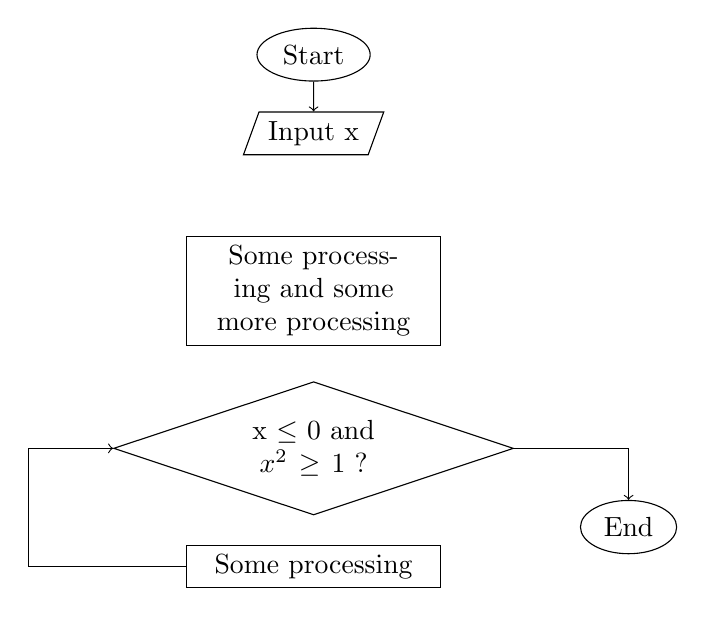
\begin{tikzpicture}
			%\draw [<->] (1,2) -- (5,4);
			%\draw (0,0) -- (5,0) -- ++(120:5) -- cycle;
			%\draw (0,1) rectangle (6,3);
			%\draw[rotate=30] (2,3) ellipse[x radius=2, y radius=1];
			%\draw (4,5) circle[radius=2];
			\node[startstop](start) {Start};
			\node[io,below of=start](input) {Input x};
			\node[normal,below of=input,yshift=-1cm](p1) {Some processing and some more processing};
			\node[decision, below of=p1,text width=2cm,yshift=-1cm](check) {x $ \leq $ 0 and $ x^2 \geq 1 $ ?};
			\node[normal,below of=check,yshift=-0.5cm](p2) {Some processing};
			\node[startstop,below of=check,right of=check,xshift=3cm](stop) {End};
			
			\draw [->] (start) -- (input);
			\draw [->] (check) -| (stop);
			\draw [->] (p2.west) -- ++(-2,0) |- (check.west);
			\end{tikzpicture}
		\end{figure}
		 
	\end{frame}
\end{document}